\documentclass{ximera}


\graphicspath{
  {./}
  {ximeraTutorial/}
  {basicPhilosophy/}
}

\newcommand{\mooculus}{\textsf{\textbf{MOOC}\textnormal{\textsf{ULUS}}}}

\usepackage{tkz-euclide}\usepackage{tikz}
\usepackage{tikz-cd}
\usetikzlibrary{arrows}
\tikzset{>=stealth,commutative diagrams/.cd,
  arrow style=tikz,diagrams={>=stealth}} %% cool arrow head
\tikzset{shorten <>/.style={ shorten >=#1, shorten <=#1 } } %% allows shorter vectors

\usetikzlibrary{backgrounds} %% for boxes around graphs
\usetikzlibrary{shapes,positioning}  %% Clouds and stars
\usetikzlibrary{matrix} %% for matrix
\usepgfplotslibrary{polar} %% for polar plots
\usepgfplotslibrary{fillbetween} %% to shade area between curves in TikZ
\usetkzobj{all}
\usepackage[makeroom]{cancel} %% for strike outs
%\usepackage{mathtools} %% for pretty underbrace % Breaks Ximera
%\usepackage{multicol}
\usepackage{pgffor} %% required for integral for loops



%% http://tex.stackexchange.com/questions/66490/drawing-a-tikz-arc-specifying-the-center
%% Draws beach ball
\tikzset{pics/carc/.style args={#1:#2:#3}{code={\draw[pic actions] (#1:#3) arc(#1:#2:#3);}}}



\usepackage{array}
\setlength{\extrarowheight}{+.1cm}
\newdimen\digitwidth
\settowidth\digitwidth{9}
\def\divrule#1#2{
\noalign{\moveright#1\digitwidth
\vbox{\hrule width#2\digitwidth}}}






\DeclareMathOperator{\arccot}{arccot}
\DeclareMathOperator{\arcsec}{arcsec}
\DeclareMathOperator{\arccsc}{arccsc}

















%%This is to help with formatting on future title pages.
\newenvironment{sectionOutcomes}{}{}

\author{Bart Snapp and Jim Talamo}


\outcome{Define orthogonal decomposition.}
\outcome{Define orthogonal and scalar projections.}
\outcome{Use the dot product in applied settings.}

\title[Dig-In:]{Projections and orthogonal decomposition}

\begin{document}
\begin{abstract}
 Projections tell us how much of one vector lies in the direction of another and are important in physical applications.
\end{abstract}
\maketitle


\section{Projections and components}

\subsection{Projections}
One of the major uses of the dot product is to let us \textit{project}
one vector in the direction of another. Conceptually, we are looking
at the ``shadow'' of one vector projected onto another, sort of like
in the case of a sundial.
\begin{image}%%https://commons.wikimedia.org/wiki/File:Perceton_sundial_-_detail.JPG
  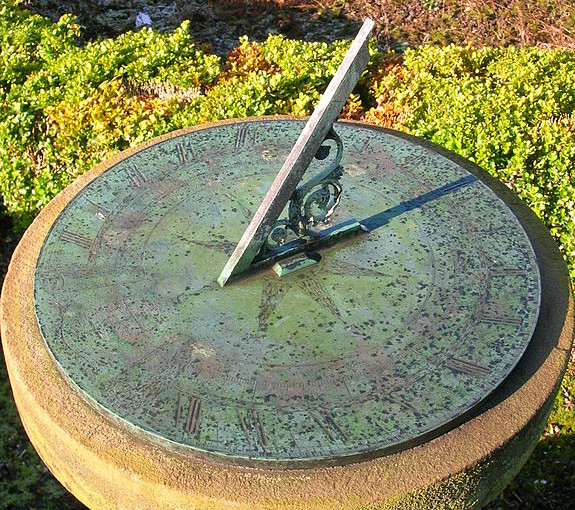
\includegraphics{sundial.jpg}
\end{image}
In essence we imagine the ``sun'' directly over a vector, casting a shadow onto another vector.
\begin{image}
  \begin{tikzpicture}
    \foreach \angle in { 270,280,...,450 }{
      \draw [ultra thick, yellow!70!orange, rotate around={\angle:(3,4)}]
      (3,3.5)--(3,3);
    };
    \draw[very thick, penColor,->] (0,0) -- (5,0);
    \draw[ultra thick,penColor4,->] (0,0) -- (3,2);
    \draw[ultra thick,penColor2,->] (0,0) -- (3,0);
    \draw[ultra thick, yellow!50!orange] (2.5,4) arc (180:360:.5);

    \draw[decoration={brace,mirror,raise=.2cm},decorate,thin] (0,0)--(3,0);
    \node at (1.5,-.5) {projection};

  \end{tikzpicture}
\end{image}






While this is good starting point for understanding orthogonal
projections, now we need the definition.

\begin{definition}
  The \textbf{orthogonal projection}\index{projection} of vector $\overset{\boldsymbol{\rightharpoonup}}{\mathbf{v}}$ in the direction
  of vector $\overset{\boldsymbol{\rightharpoonup}}{\mathbf{w}}$ is a new vector denoted
  $\mathbf{proj}_{\overset{\boldsymbol{\rightharpoonup}}{\mathbf{w}}}(\overset{\boldsymbol{\rightharpoonup}}{\mathbf{v}})$
  \begin{image}
    \begin{tikzpicture}
      \draw[dashed] (-.5,-.5) -- (3.5,3.5);
      \draw[ultra thick,penColor4,->] (0,0) -- (3,1);
      \draw[ultra thick,penColor2,->] (-0,0) -- (0.707,0.707);
      %\draw[textColor, dashed] (3,1) -- (2,2);
      \node[below] at (1.5, 0.5) [penColor4] {$\overset{\boldsymbol{\rightharpoonup}}{\mathbf{v}}$};
      \node at (0.2, .5) [penColor2] {$\overset{\boldsymbol{\rightharpoonup}}{\mathbf{w}}$};
    \end{tikzpicture}
    \qquad
    \begin{tikzpicture}
      \draw[textColor, dashed] (3,1) -- (2,2);
      \draw[textColor, thin] (2.2,1.8) -- (2,1.6)--(1.8,1.8);
      \draw[draw=none] (-.5,-.5) -- (3.5,3.5);
      \draw[very thick, penColor,->] (0,0) -- (2,2);
      \draw[ultra thick,penColor4,->] (0,0) -- (3,1);
      \draw[ultra thick,penColor2,->] (-0,0) -- (0.707,0.707);
      %\node[above] at (1.5, 0.5) [penColor] {$\overset{\boldsymbol{\rightharpoonup}}{\mathbf{v}}$};
      %\node at (0.2, .5) [penColor2] {$\overset{\boldsymbol{\rightharpoonup}}{\mathbf{w}}$};
      \node[above left] at (1, 1) [penColor] {$\mathbf{proj}_{\overset{\boldsymbol{\rightharpoonup}}{\mathbf{w}}}(\overset{\boldsymbol{\rightharpoonup}}{\mathbf{v}})$};
    \end{tikzpicture}
  \end{image}
  that lies on the line containing $\overset{\boldsymbol{\rightharpoonup}}{\mathbf{w}}$, with the vector
  $\mathbf{proj}_{\overset{\boldsymbol{\rightharpoonup}}{\mathbf{w}}}(\overset{\boldsymbol{\rightharpoonup}}{\mathbf{v}}) - \overset{\boldsymbol{\rightharpoonup}}{\mathbf{v}}$ perpendicular to $\overset{\boldsymbol{\rightharpoonup}}{\mathbf{w}}$.
  \begin{onlineOnly}
    Below we see vectors $\overset{\boldsymbol{\rightharpoonup}}{\mathbf{v}}$ and $\overset{\boldsymbol{\rightharpoonup}}{\mathbf{w}}$ along with
    $\mathbf{proj}_{\overset{\boldsymbol{\rightharpoonup}}{\mathbf{w}}}(\overset{\boldsymbol{\rightharpoonup}}{\mathbf{v}})$. Move the tips of vectors $\overset{\boldsymbol{\rightharpoonup}}{\mathbf{v}}$ and
    $\overset{\boldsymbol{\rightharpoonup}}{\mathbf{w}}$ to help you understand $\mathbf{proj}_{\overset{\boldsymbol{\rightharpoonup}}{\mathbf{w}}}(\overset{\boldsymbol{\rightharpoonup}}{\mathbf{v}})$.
    \begin{center}
      \geogebra{f8bqsRAz}{800}{600}
    \end{center}
\end{onlineOnly}
\end{definition}


\begin{question}
  Consider the vector $\overset{\boldsymbol{\rightharpoonup}}{\mathbf{v}}=\left< 3,2,1 \right>$ and the vector $\boldsymbol{\hat{\imath}} =
  \left< 1,0,0 \right>$.  Compute $\mathbf{proj}_{\boldsymbol{\hat{\imath}}}(\overset{\boldsymbol{\rightharpoonup}}{\mathbf{v}})$.
  \begin{hint}
    Draw a picture.
  \end{hint}
  \begin{prompt}
    \[
    \mathbf{proj}_{\boldsymbol{\hat{\imath}}}(\overset{\boldsymbol{\rightharpoonup}}{\mathbf{v}}) = \left< \answer{3},\answer{0},\answer{0} \right>
    \]
  \end{prompt}
  \begin{question}
    Let $\overset{\boldsymbol{\rightharpoonup}}{\mathbf{v}} = \left< 1,1 \right>$ and $\overset{\boldsymbol{\rightharpoonup}}{\mathbf{w}}= \left< -1,1 \right>$. Compute
    $\mathbf{proj}_{\overset{\boldsymbol{\rightharpoonup}}{\mathbf{w}}}(\overset{\boldsymbol{\rightharpoonup}}{\mathbf{v}})$.
    \begin{hint}
      Draw a picture.
    \end{hint}
      \begin{prompt}
        \[
        \mathbf{proj}_{\overset{\boldsymbol{\rightharpoonup}}{\mathbf{w}}}(\overset{\boldsymbol{\rightharpoonup}}{\mathbf{v}}) = \left< \answer{0},\answer{0} \right>
        \]
      \end{prompt}
  \end{question}
\end{question}

To compute the projection of one vector along another, we use the dot
product.


\begin{theorem}
  Given two vectors $\overset{\boldsymbol{\rightharpoonup}}{\mathbf{v}}$ and $\overset{\boldsymbol{\rightharpoonup}}{\mathbf{w}}$
  \[
  \mathbf{proj}_{\overset{\boldsymbol{\rightharpoonup}}{\mathbf{w}}}(\overset{\boldsymbol{\rightharpoonup}}{\mathbf{v}})
  =\left(\frac{\overset{\boldsymbol{\rightharpoonup}}{\mathbf{v}} \bullet \overset{\boldsymbol{\rightharpoonup}}{\mathbf{w}}}{|\overset{\boldsymbol{\rightharpoonup}}{\mathbf{w}}|^2}\right) \overset{\boldsymbol{\rightharpoonup}}{\mathbf{w}}
  =\left(\frac{\overset{\boldsymbol{\rightharpoonup}}{\mathbf{v}} \bullet \overset{\boldsymbol{\rightharpoonup}}{\mathbf{w}}}{\overset{\boldsymbol{\rightharpoonup}}{\mathbf{w}} \bullet \overset{\boldsymbol{\rightharpoonup}}{\mathbf{w}}}\right) \overset{\boldsymbol{\rightharpoonup}}{\mathbf{w}}.
  \]
  \begin{explanation}
    First, note that the direction of $\mathbf{proj}_{\overset{\boldsymbol{\rightharpoonup}}{\mathbf{w}}}(\overset{\boldsymbol{\rightharpoonup}}{\mathbf{v}})$ is given by
    \[
    \frac{\overset{\boldsymbol{\rightharpoonup}}{\mathbf{w}}}{|\overset{\boldsymbol{\rightharpoonup}}{\mathbf{w}}|}
    \]
    and the magnitude of $\mathbf{proj}_{\overset{\boldsymbol{\rightharpoonup}}{\mathbf{w}}}(\overset{\boldsymbol{\rightharpoonup}}{\mathbf{v}})$ is given by
    \[
    |\mathbf{proj}_{\overset{\boldsymbol{\rightharpoonup}}{\mathbf{w}}}(\overset{\boldsymbol{\rightharpoonup}}{\mathbf{v}})| = |\overset{\boldsymbol{\rightharpoonup}}{\mathbf{v}}|\cdot \left| \answer[given]{\cos(\theta)}\right|.
    \]
    \begin{image}
      \begin{tikzpicture}
        \draw (.5,.1) arc[radius=.5cm,start angle=11.3,end angle=56.3];
        \draw[->,ultra thick,penColor] (0,0) -- (5,1);
        \draw[->,ultra thick,penColor2] (0,0) -- (2,3);
        \draw[thin] (2.46,.71)--(2.25,.67)--(2.29,0.46);
        \draw[dashed] (2,3) -- (2.5,.5);
        \node[below,penColor] at (3.75,.75) {$\overset{\boldsymbol{\rightharpoonup}}{\mathbf{w}}$}; %% <a,b>
        \node[above left,penColor2] at (1,1.5) {$\overset{\boldsymbol{\rightharpoonup}}{\mathbf{v}}$}; %% <c,d>
        \node[above right] at (.4,.2) {$\theta$}; %% <c,d>
        \draw[decoration={brace,mirror,raise=.2cm},decorate,thin] (0,0)--(2.5,.5);
        \node at (1.25,-.25) {$\cos(\theta)$};
      \end{tikzpicture}
    \end{image}
    Now
    \[
    \mathbf{proj}_{\overset{\boldsymbol{\rightharpoonup}}{\mathbf{w}}}(\overset{\boldsymbol{\rightharpoonup}}{\mathbf{v}}) = \mathrm{direction}\cdot\mathrm{magnitude},
    \]
    where
    \[
    \mathrm{direction} = \pm \frac{\overset{\boldsymbol{\rightharpoonup}}{\mathbf{w}}}{|\overset{\boldsymbol{\rightharpoonup}}{\mathbf{w}}|}
    \]
    has a positive sign if $0<\theta< \pi/2$, and a negative sign if
    $\pi/2< \theta< \pi$. Also,
    \[
    \mathrm{magnitude} = |\overset{\boldsymbol{\rightharpoonup}}{\mathbf{v}}|\cdot\left|\answer[given]{\cos(\theta)}\right|.
    \]
    Multiplying direction and magnitude we find the following.
    \begin{align*}
      &= \frac{\overset{\boldsymbol{\rightharpoonup}}{\mathbf{w}}}{|\overset{\boldsymbol{\rightharpoonup}}{\mathbf{w}}|^2}\cdot |\overset{\boldsymbol{\rightharpoonup}}{\mathbf{w}}|\cdot |\overset{\boldsymbol{\rightharpoonup}}{\mathbf{v}}|\cdot\answer[given]{\cos(\theta)}\\
      &= \left(\frac{\overset{\boldsymbol{\rightharpoonup}}{\mathbf{v}} \bullet \overset{\boldsymbol{\rightharpoonup}}{\mathbf{w}}}{|\overset{\boldsymbol{\rightharpoonup}}{\mathbf{w}}|^2}\right) \overset{\boldsymbol{\rightharpoonup}}{\mathbf{w}}\\
      &=\left(\frac{\overset{\boldsymbol{\rightharpoonup}}{\mathbf{v}} \bullet \overset{\boldsymbol{\rightharpoonup}}{\mathbf{w}}}{\overset{\boldsymbol{\rightharpoonup}}{\mathbf{w}} \bullet \overset{\boldsymbol{\rightharpoonup}}{\mathbf{w}}}\right) \overset{\boldsymbol{\rightharpoonup}}{\mathbf{w}}.
    \end{align*}
    Notice that the sign of the direction is the sign of cosine, so we simply remove the absolute value from the cosine.
  \end{explanation}
\end{theorem}


\begin{question}
  Find the projection of the vector $\overset{\boldsymbol{\rightharpoonup}}{\mathbf{v}} = \left< 2,3,1 \right>$ in the
  direction of the vector $\overset{\boldsymbol{\rightharpoonup}}{\mathbf{w}} = \left< 3,-1,1 \right>$.
  \begin{prompt}
  \[
  \mathbf{proj}_{\overset{\boldsymbol{\rightharpoonup}}{\mathbf{w}}}(\overset{\boldsymbol{\rightharpoonup}}{\mathbf{v}}) = \left< \answer{\frac{12}{11}},\answer{\frac{-4}{11}},\answer{\frac{4}{11}} \right>
  \]
  \end{prompt}
\end{question}

\begin{question}
  Let $\overset{\boldsymbol{\rightharpoonup}}{\mathbf{v}}$ and $\overset{\boldsymbol{\rightharpoonup}}{\mathbf{w}}$ be nonzero vectors in $\mathbb{R}^2$. Let $k\ge
  1$. Select all statements that must be true.
  \begin{selectAll}
    \choice{$\mathbf{proj}_{\overset{\boldsymbol{\rightharpoonup}}{\mathbf{w}}}(\overset{\boldsymbol{\rightharpoonup}}{\mathbf{v}})=\mathbf{proj}_{\overset{\boldsymbol{\rightharpoonup}}{\mathbf{v}}}(\overset{\boldsymbol{\rightharpoonup}}{\mathbf{w}})$}
    \choice[correct]{$|\mathbf{proj}_{\overset{\boldsymbol{\rightharpoonup}}{\mathbf{w}}}(\overset{\boldsymbol{\rightharpoonup}}{\mathbf{v}})|\le |\overset{\boldsymbol{\rightharpoonup}}{\mathbf{v}}|$}
    \choice{$|\mathbf{proj}_{\overset{\boldsymbol{\rightharpoonup}}{\mathbf{w}}}(\overset{\boldsymbol{\rightharpoonup}}{\mathbf{v}})|\le |\overset{\boldsymbol{\rightharpoonup}}{\mathbf{w}}|$}
    \choice[correct]{$|\mathbf{proj}_{\overset{\boldsymbol{\rightharpoonup}}{\mathbf{w}}}(\overset{\boldsymbol{\rightharpoonup}}{\mathbf{v}})|\le |\mathbf{proj}_{\overset{\boldsymbol{\rightharpoonup}}{\mathbf{w}}}(k\cdot \overset{\boldsymbol{\rightharpoonup}}{\mathbf{v}})|$}
    \choice{$|\mathbf{proj}_{\overset{\boldsymbol{\rightharpoonup}}{\mathbf{w}}}(k\cdot \overset{\boldsymbol{\rightharpoonup}}{\mathbf{v}})|\le |\mathbf{proj}_{\overset{\boldsymbol{\rightharpoonup}}{\mathbf{w}}}(\overset{\boldsymbol{\rightharpoonup}}{\mathbf{v}})|$}
    \choice[correct]{$|\mathbf{proj}_{\overset{\boldsymbol{\rightharpoonup}}{\mathbf{w}}}(\overset{\boldsymbol{\rightharpoonup}}{\mathbf{v}})|\le |\mathbf{proj}_{k\cdot \overset{\boldsymbol{\rightharpoonup}}{\mathbf{w}}}(\overset{\boldsymbol{\rightharpoonup}}{\mathbf{v}})|$}
    \choice[correct]{$|\mathbf{proj}_{k\cdot \overset{\boldsymbol{\rightharpoonup}}{\mathbf{w}}}(\overset{\boldsymbol{\rightharpoonup}}{\mathbf{v}})|\le |\mathbf{proj}_{\overset{\boldsymbol{\rightharpoonup}}{\mathbf{w}}}(\overset{\boldsymbol{\rightharpoonup}}{\mathbf{v}})|$}
  \end{selectAll}
\end{question}



\subsection{Components}
Scalar components compute ``how much'' of a vector is pointing in a
particular direction.
\begin{definition}
  Let $\overset{\boldsymbol{\rightharpoonup}}{\mathbf{v}}$ and $\overset{\boldsymbol{\rightharpoonup}}{\mathbf{w}}$ be vectors and let $0\le\theta\le\pi$ be
  the angle between them.  The \textbf{scalar component}\index{component}
  in the direction of $\overset{\boldsymbol{\rightharpoonup}}{\mathbf{w}}$ of vector $\overset{\boldsymbol{\rightharpoonup}}{\mathbf{v}}$ is denoted
  \[
  scal_{\overset{\boldsymbol{\rightharpoonup}}{\mathbf{w}}}(\overset{\boldsymbol{\rightharpoonup}}{\mathbf{v}})=
  \begin{cases}
    |\mathbf{proj}_{\overset{\boldsymbol{\rightharpoonup}}{\mathbf{w}}}(\overset{\boldsymbol{\rightharpoonup}}{\mathbf{v}})| &\text{when $0\le\theta\le \pi/2$}\\
    -|\mathbf{proj}_{\overset{\boldsymbol{\rightharpoonup}}{\mathbf{w}}}(\overset{\boldsymbol{\rightharpoonup}}{\mathbf{v}})| &\text{when $\pi/2<\theta\le \pi$.}
  \end{cases}
  \]
\end{definition}



\begin{question}
  Let $\overset{\boldsymbol{\rightharpoonup}}{\mathbf{v}} = \left< 3,-2,1 \right>$. Compute $scal_{\boldsymbol{\hat{\imath}}}(\overset{\boldsymbol{\rightharpoonup}}{\mathbf{v}})$.
  \begin{prompt}
    \[
    scal_{\boldsymbol{\hat{\imath}}}(\overset{\boldsymbol{\rightharpoonup}}{\mathbf{v}}) = \answer{3}
    \]
  \end{prompt}
  \begin{question}
    Compute $scal_{\boldsymbol{\hat{\jmath}}}(\overset{\boldsymbol{\rightharpoonup}}{\mathbf{v}})$.
    \begin{prompt}
      \[
      scal_{\boldsymbol{\hat{\jmath}}}(\overset{\boldsymbol{\rightharpoonup}}{\mathbf{v}}) = \answer{-2}
      \]
    \end{prompt}
    \begin{question}
      Compute $scal_{\boldsymbol{\hat{k}}}(\overset{\boldsymbol{\rightharpoonup}}{\mathbf{v}})$.
      \begin{prompt}
        \[
        scal_{\boldsymbol{\hat{k}}}(\overset{\boldsymbol{\rightharpoonup}}{\mathbf{v}}) = \answer{1}
        \]
      \end{prompt}
    \end{question}
  \end{question}
\end{question}

To compute the scalar component of a vector in the direction of
another, you use the dot product.

\begin{theorem}
  Given two vectors, $\overset{\boldsymbol{\rightharpoonup}}{\mathbf{v}}$ and $\overset{\boldsymbol{\rightharpoonup}}{\mathbf{w}}$,
  \[
  scal_{\overset{\boldsymbol{\rightharpoonup}}{\mathbf{w}}}(\overset{\boldsymbol{\rightharpoonup}}{\mathbf{v}}) =\frac{\overset{\boldsymbol{\rightharpoonup}}{\mathbf{v}} \bullet \overset{\boldsymbol{\rightharpoonup}}{\mathbf{w}}}{|\overset{\boldsymbol{\rightharpoonup}}{\mathbf{w}}|}.
  \]
\end{theorem}

\begin{question}
  Let $\overset{\boldsymbol{\rightharpoonup}}{\mathbf{v}}$ and $\overset{\boldsymbol{\rightharpoonup}}{\mathbf{w}}$ be nonzero vectors and let $\theta$ be
  the angle between them. Which of the following are true?
  \begin{selectAll}
    \choice{$|\mathbf{proj}_{\overset{\boldsymbol{\rightharpoonup}}{\mathbf{w}}}(\overset{\boldsymbol{\rightharpoonup}}{\mathbf{v}})| = scal_{\overset{\boldsymbol{\rightharpoonup}}{\mathbf{w}}}(\overset{\boldsymbol{\rightharpoonup}}{\mathbf{v}})$}
    \choice[correct]{$|\mathbf{proj}_{\overset{\boldsymbol{\rightharpoonup}}{\mathbf{w}}}(\overset{\boldsymbol{\rightharpoonup}}{\mathbf{v}})| = |scal_{\overset{\boldsymbol{\rightharpoonup}}{\mathbf{w}}}(\overset{\boldsymbol{\rightharpoonup}}{\mathbf{v}})|$}
    \choice[correct]{$\mathbf{proj}_{\overset{\boldsymbol{\rightharpoonup}}{\mathbf{w}}}(\overset{\boldsymbol{\rightharpoonup}}{\mathbf{v}}) =|\overset{\boldsymbol{\rightharpoonup}}{\mathbf{v}}|\cos(\theta)\left(\frac{\overset{\boldsymbol{\rightharpoonup}}{\mathbf{w}}}{|\overset{\boldsymbol{\rightharpoonup}}{\mathbf{w}}|}\right)$}
    \choice[correct]{$scal_{\overset{\boldsymbol{\rightharpoonup}}{\mathbf{w}}}(\overset{\boldsymbol{\rightharpoonup}}{\mathbf{v}}) = |\overset{\boldsymbol{\rightharpoonup}}{\mathbf{v}}|\cos(\theta)$}
  \end{selectAll}
\end{question}



\subsection{Orthogonal decomposition}


Given any vector $\overset{\boldsymbol{\rightharpoonup}}{\mathbf{v}}$ in $\mathbb{R}^2$, we can always write it as
\[
\overset{\boldsymbol{\rightharpoonup}}{\mathbf{v}} = a\boldsymbol{\hat{\imath}} + b\boldsymbol{\hat{\jmath}}
\]
for some real numbers $a$ and $b$.  Here we've broken $\overset{\boldsymbol{\rightharpoonup}}{\mathbf{v}}$ into
the sum of two orthogonal vectors --- in particular, vectors parallel to
$\boldsymbol{\hat{\imath}}$ and $\boldsymbol{\hat{\jmath}}$. In fact, given a vector $\overset{\boldsymbol{\rightharpoonup}}{\mathbf{v}}$ and another
vector $\overset{\boldsymbol{\rightharpoonup}}{\mathbf{w}}$ you can always break $\overset{\boldsymbol{\rightharpoonup}}{\mathbf{v}}$ into a sum of two
vectors, one of which is parallel to $\overset{\boldsymbol{\rightharpoonup}}{\mathbf{w}}$ and another that is
perpendicular to $\overset{\boldsymbol{\rightharpoonup}}{\mathbf{w}}$. Such a sum is called an \textit{orthogonal
  decomposition}.
\begin{onlineOnly}
  Move the point around to see various orthogonal decompositions of
  vector $\overset{\boldsymbol{\rightharpoonup}}{\mathbf{v}}$.
  \begin{center}
    \geogebra{juszKc6k}{800}{600}
  \end{center}
\end{onlineOnly}

\begin{definition}
Let $\overset{\boldsymbol{\rightharpoonup}}{\mathbf{v}}$ and $\overset{\boldsymbol{\rightharpoonup}}{\mathbf{w}}$ be vectors. The \textbf{orthogonal
  decomposition} of $\overset{\boldsymbol{\rightharpoonup}}{\mathbf{v}}$ in terms of $\overset{\boldsymbol{\rightharpoonup}}{\mathbf{w}}$ is the sum
\[
\overset{\boldsymbol{\rightharpoonup}}{\mathbf{v}} = \underbrace{\mathbf{proj}_{\overset{\boldsymbol{\rightharpoonup}}{\mathbf{w}}}(\overset{\boldsymbol{\rightharpoonup}}{\mathbf{v}})}_{\parallel \overset{\boldsymbol{\rightharpoonup}}{\mathbf{w}}} +  (\underbrace{\overset{\boldsymbol{\rightharpoonup}}{\mathbf{v}}-\mathbf{proj}_{\overset{\boldsymbol{\rightharpoonup}}{\mathbf{w}}}(\overset{\boldsymbol{\rightharpoonup}}{\mathbf{v}})}_{\perp \overset{\boldsymbol{\rightharpoonup}}{\mathbf{w}}}),
\]
where $\overset{\boldsymbol{\rightharpoonup}}{\mathbf{x}} \parallel \overset{\boldsymbol{\rightharpoonup}}{\mathbf{y}}$ means that ``$\overset{\boldsymbol{\rightharpoonup}}{\mathbf{x}}$ is parallel
to $\overset{\boldsymbol{\rightharpoonup}}{\mathbf{y}}$'' and $\overset{\boldsymbol{\rightharpoonup}}{\mathbf{x}} \perp\overset{\boldsymbol{\rightharpoonup}}{\mathbf{y}}$ means that ``$\overset{\boldsymbol{\rightharpoonup}}{\mathbf{x}}$ is
perpendicular to $\overset{\boldsymbol{\rightharpoonup}}{\mathbf{y}}$''.
\end{definition}














\end{document}
